% $Id: template.tex 11 2007-04-03 22:25:53Z jpeltier $

\documentclass{vgtc} 

\ifpdf%                                % if we use pdflatex
  \pdfoutput=1\relax                   % create PDFs from pdfLaTeX
  \pdfcompresslevel=9                  % PDF Compression
  \pdfoptionpdfminorversion=7          % create PDF 1.7
  \ExecuteOptions{pdftex}
  \usepackage{graphicx}                % allow us to embed graphics files
  \DeclareGraphicsExtensions{.pdf,.png,.jpg,.jpeg} % for pdflatex we expect .pdf, .png, or .jpg files
\else%                                 % else we use pure latex
  \ExecuteOptions{dvips}
  \usepackage{graphicx}                % allow us to embed graphics files
  \DeclareGraphicsExtensions{.eps}     % for pure latex we expect eps files
\fi%

%% it is recomended to use ``\autoref{sec:bla}'' instead of ``Fig.~\ref{sec:bla}''
\graphicspath{{figures/}{pictures/}{images/}{./}} % where to search for the images

\usepackage{microtype}                 % use micro-typography (slightly more compact, better to read)
\PassOptionsToPackage{warn}{textcomp}  % to address font issues with \textrightarrow
\usepackage{textcomp}                  % use better special symbols
\usepackage{mathptmx}                  % use matching math font
\usepackage{times}                     % we use Times as the main font
\renewcommand*\ttdefault{txtt}         % a nicer typewriter font
\usepackage{cite}                      % needed to automatically sort the references
\usepackage{hyperref}

%%Title
\title{College Mobility Explorer}

%% Author and Affiliation
\author{Ariel Levy\thanks{e-mail: aslevy@mit.edu}\\ %
        \scriptsize Massachusetts Institute of Technology %
\and Erica Zhou\thanks{e-mail: ezhou@mit.edu}\\ %
     \scriptsize Massachusetts Institute of Technology}
 
%% Abstract section.
\abstract{In the last few years, the college application process has become increasingly focused on competitive admission to elite schools with widespread brand recognition, where high income families have a distinct advantage. Highlighting schools based on opportunity for economic mobility, especially for low income families, is an under-served use case with existing college exploration and ranking tools. In this paper, we present College Mobility Explorer, an interface to inform students of college options based on institutional characteristics and student desires, while prioritizing economic success post-graduation as an outcome. The interface allows students to select target values for different features of schools and weight how desirable those features are. The College Mobility Explorer then calculates a match score for each potential school based on user customization and displays a ranked list of colleges that most closely align with student desires. The College Mobility Explorer also displays a scatter plot of all potential schools based on both match score and mobility score, a measure of projected post-graduate economic rank for users. Thus, the platform allows for both the discovery of individual schools for students to make more informed application decisions and the depiction of overall trends of post-graduate mobility based on several different features of colleges.} 

% %% ACM Computing Classification System (CCS). 
% \CCScatlist{
%   \CCScatTwelve{Human-centered computing}{Visu\-al\-iza\-tion}{Visualization design and evaluation methods}{}  
%   \CCScatTwelve{User Interfaces}{User Interfaces}{Graphical user interfaces (GUI)}{};
%   \CCScatTwelve{Information Interfaces and Presentation}{Miscellaneous}{}{}
% }

%% Copyright space is enabled by default as required by guidelines.
%% It is disabled by the 'review' option or via the following command:
% \nocopyrightspace

%%%%%%%%%%%%%%%%%%%%%%%%%%%%%%%%%%%%%%%%%%%%%%%%%%%%%%%%%%%%%%%%
%%%%%%%%%%%%%%%%%%%%%% START OF THE PAPER %%%%%%%%%%%%%%%%%%%%%%
%%%%%%%%%%%%%%%%%%%%%%%%%%%%%%%%%%%%%%%%%%%%%%%%%%%%%%%%%%%%%%%%%

\begin{document}
\maketitle

\section{Introduction}
In the last several years, the college application process has become increasing focused on competitive admission to elite schools with widespread brand recognition. Recent news, such as the college admission bribery scandal, has highlighted how students from high income families have a distinct advantage in accessing these elite schools. There has been a lack of attention towards the colleges in America that actually provide the most opportunities for economic mobility to their students, let alone tools to make this information accessible and actionable to prospective college students from low-income families. 

The most popular existing platforms available to students to explore their college options include high-school specific admissions likelihood tools like Naviance and college ranking organizations like Niche and the U.S. News \& World Report. Naviance allows students to find college options given their GPA and SAT Score, but it focuses on likelihood of admission as the primary outcome of application rather than value received from higher education as a whole. It tends to highlight schools with low admission rate to students rather than provide opportunities to discover less well-known schools that might better serve students’ needs. Niche ranks colleges with an algorithm that most heavily weights factors of admission rate, professor quality, and student ratings of the schools. U.S. News \& World Report is well-known for its ``Best Colleges'' list which ranks schools based on academic quality. It also has a ``Best Value Schools'' list that ranks based on ratio of tuition to education quality as measured by the ``Best Colleges'' ranking and financial aid. However, this list is also not focused on post-graduation outcomes and still favors elite institutions.

In this paper, we present College Mobility Explorer, a platform to discover college options based on institutional characteristics and student desires, while prioritizing potential economic mobility post-graduation as an outcome. The interactive interface of the platform allows students to select target values for different features of schools and weight how desirable those features are. The College Mobility Explorer then calculates a match score for each potential school based on user customization and displays a ranked list of colleges that most closely align with student desires. The College Mobility Explorer also displays a scatter plot of all potential schools based on both match score and mobility score, a measure of projected post-graduate economic rank for users. This illustrates each school’s individual trade-off between mobility opportunity and match for desired features, and it also shows the general pattern of the whole set of schools.

Thus, the platform allows for both the discovery of individual schools and the understanding of overall trends of post-graduate mobility based on different features of colleges. The discovery of individual schools results from the student’s desires rather than determinations of outside institutions, and the scatter plot highlights schools with the most potential for economic success rather than the lowest admission rates. Therefore, students, especially those from low-income families, can make more informed application decisions.

\section{Related Work}
The College Mobility Explorer is visualizing the publicly-available dataset ``Mobility Report Cards: The Role of Colleges in Intergenerational Mobility'' produced by the Opportunity Insights research team \cite{mobility}. The major related work to the College Mobility Explorer based on this dataset is an article and series of visualizations produced by the New York Times \cite{gregor_aisch_2017}.

The interactive New York Times article on this dataset presents several static visualizations showing overall patterns in categories of schools for different income brackets. These are focused on trends in the effect of selectivity of the school on mobility rather than on the specific schools themselves. The interface also presents ranked lists of schools that do well or poorly on different mobility metrics, which highlights specific schools but only considers a few specific features. The interactivity of the interface allows users to enter a specific school by name and see where the school stands on the ranked lists, as well as see further static visualizations on how the school compares to peer institutions on several different economic mobility and diversity metrics. However, there is not much opportunity for discovery of previously unknown schools to see these assessments.

\section{Dataset}
The major dataset for this visualization comes from the Opportunity Insights organization, and  specificlaly from Chetty et. al.'s ``Mobility Report Cards: The Role of Colleges in Intergenerational Mobility'' \cite{mobility} . This dataset focuses on intergenerational income mobility for colleges, and the report discusses access to colleges by income, outcomes for each college conditional on income, rates of upward mobility, and the change in income distribution at colleges over time. In this report, mobility is defined as defined as the percentage chance of moving from the bottom to the top quintile.

Additionally, the general college information comes from a table of college characteristics, which was developed using the US Department of Education's Integrated Postsecondary Education Data System (IPEDS) database and College scorecard.

\section{Methodology}
As seen in \autoref{fig:overview}, the interface consists of a section containing filters and sliders representing features of different colleges, a selector for parental income, a list of the top 100 college matches, and a scatter plot depicting income mobility versus match between student preferences and college characteristics. Additionally, clicking on an individual college brings up more detailed information and visualizations about the school. This section describes our definition of mobility as well as the specific visualization techniques and algorithms used to generate each section of the platform.

\begin{figure}[tbh]
 \centering
 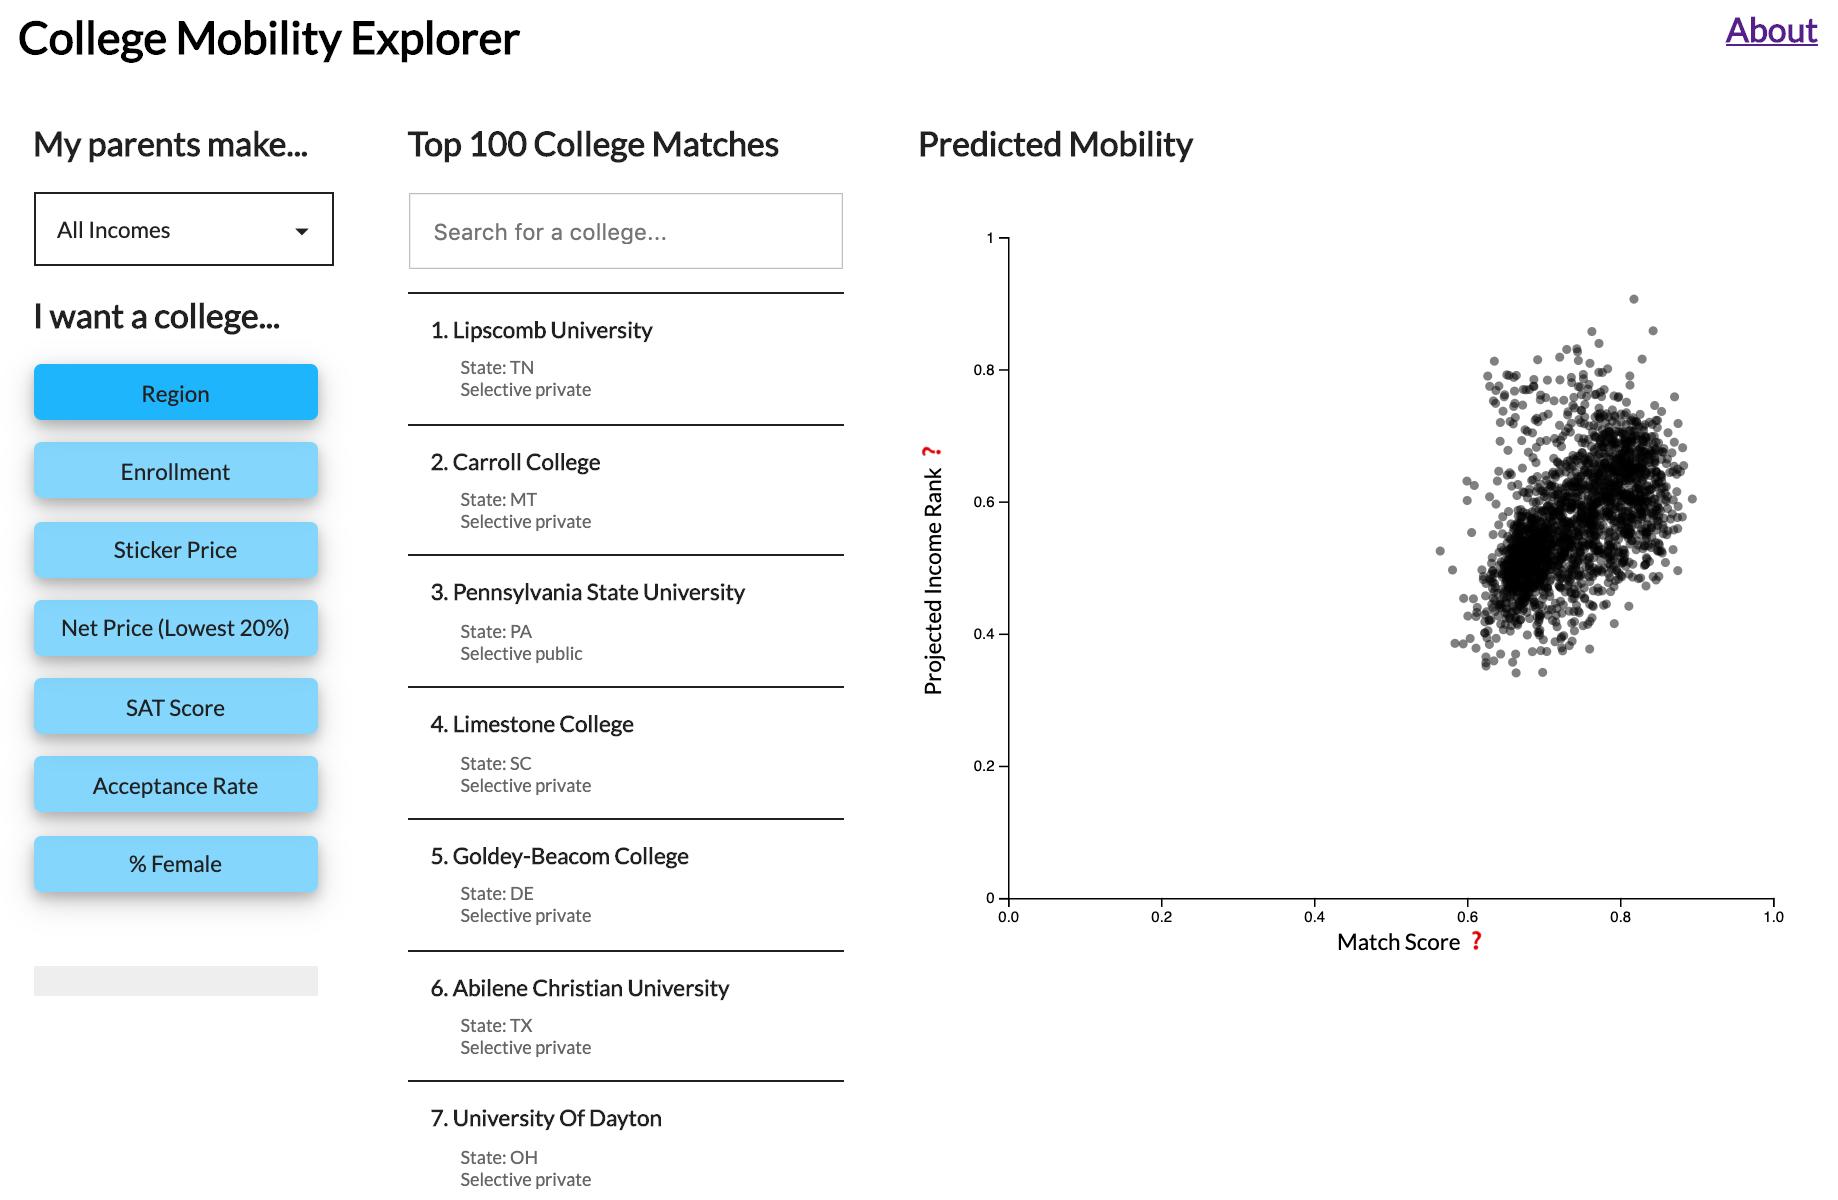
\includegraphics[width=\columnwidth]{overview.png}
 \caption{An overview of the College Mobility Explorer interface upon initialization.}
 \label{fig:overview}
\end{figure}

\subsection{Mobility}
There are many possible ways to define ``mobility'' achieved from attending a specific college. As mentioned in Section 3, the Opportunity Insights organization considers this measure as the percentage of students moving from the bottom to top income quintile. However, the College Mobility Explorer aims to show students opportunities specific to them, so mobility is approximated as a percentile rank of students' incomes conditional on their parents starting in a given income quintile.

This measure ends up giving an objective measure of income as opposed to a specific ``mobility'' measure for each student. However, it is much more specific to each income quintile and allows for a standardized measure to be used for every quintile and every college. Additionally, it still allows for comparison between different colleges, and the change between the starting quintile and the ending income gives an idea of economic mobility. In this way, students can see a more fine-grained and objective predicted income for students like them, and the tool becomes more personalized to their specific situations. 

\subsection{Filters \& Sliders}
The filters and sliders depict various options for students to select their desired features in a college, as well as how important these features are to them. The features are both categorical, such as location (region), and quantitative, such as acceptance rate and cost. They are depicted as clickable buttons, where clicking on each button highlights it and brings up the options for that specific filter. Using this method allows students to see all of the possible features they can consider, as well as select one and see in real-time how this affects the colleges that suit them most closely.

The categorical region filter acts as a binary filter and limits the schools depicted in both the top matches and in the scatter plot. Thus, for these features, a college either meets the requirements and is considered, or it does not and disappears from the scatter plot. In contrast, clicking on a quantitative feature brings up two sliders: one for the target value of that feature, and one for the importance of that feature in overall college selection. From a student's selections, we are able to objectively see how much schools differ from his individual preferences, and we use this to tailor results uniquely to each student.

The College Mobility Explorer includes the following features for students to consider:
\begin{itemize}
    \item \textit{Region} - Northeast, Midwest, South, and/or West (can select multiple); binary filter
    \item \textit{Enrollment} - undergraduate enrollment (full \& part-time)
    \item \textit{Sticker Price} - average annual cost of attendance (including room \& board and other fees)
    \item \textit{Net Price} - average annual cost of attendance for students in the lowest income quintile; an approximation for financial aid
    \item \textit{SAT Score} - average SAT score (out of 1600)
    \item \textit{Acceptance Rate}
    \item \textit{\% Female} -  gender ratio for undergraduate students
\end{itemize}

\subsection{Income Selector}
The income selector allows users to select their own income quintiles and see what effect their starting quintile has on their predicted income after college. It takes the form of a drop-down menu, so students can select their particular income quintile, and researchers can also compare the income distributions given different starting income quintiles. The income selector also includes the overall ranking for all income quintiles to give an overall idea of income resulting from each college.

\subsection{Top Matches}
The top college matches for each student are generated for each student based on the match between their desired features and the features of each institution. After filtering out schools that do not fulfill the requirements of the categorical variables, in this case region, the ``match score'' is calculated for each school. To calculate the match for each school, we consider the difference between each of the college's features and the student's desired features, as well as how important each feature is to the student:
\begin{equation}
    score_{school} = \sum_{f \in features} w_{f} \cdot (1-|v_{f, desired} - v_{f, school}|)
    \label{eqn:avg}
\end{equation}
where $w$ is the weight (\textit{importance} in the feature selection dropdown), $v_{f, desired}$ is the students desired value (\textit{target value} in the feature selection dropdown), and $v_{f,school}$ is the value of each feature that this college offers.

Additionally, the score is normalized to the maximum possible score given the selected weights and only using features with existing data. This accounts for the case where a student weights every feature as unimportant, which would otherwise just generate a low match score for every school. Additionally, it normalizes out missing data, as opposed to just lowering a school's score if data is missing. Accordingly, we modify \autoref{eqn:avg} as follows:
\begin{equation}
    score_{school} = \sum_{f \in features,f!=\ null} w_{f} \cdot (1-|v_{f, desired} - v_{f, school}|)
\end{equation}
\begin{equation}    
    max\_score_{school} = \sum_{f \in features,school[f]!=null} w_{f}
\end{equation}
\begin{equation}    
    match\_score_{school} = \frac{score_{school}}{max\_score_{school}}
    \label{eqn:match}
\end{equation}
\autoref{eqn:avg} gives the final match score calculated for each school, which changes automatically upon adjusting a desired feature or importance.

The ``Top 100 College Matches'' list gives the top 100 schools by match score for a given set of desired features. It also contains a search bar that allows searching for specific colleges (in the top 100) by name, and clicking on a specific college shows its place on the mobility chart and brings up more information about the school.

\subsection{Scatter Plot}
The scatter plot is the main depiction of mobility for different colleges. Each point represents a specific college, where its match score is on the x-axis and average income rank after college for its students is on the y-axis. The use of a scatter plot makes it easy to view all schools simultaneously and visualize the trade-offs between potential mobility and desired college features.

\autoref{fig:cuny} depicts the scatter plot visualization resulting from a specific selection of desired features and weights. The scatter plot depicts the starting income quintile in blue, and it allows for selection of a specific school (shown in yellow) by clicking on it in either the colleges list or on the plot itself. The difference between the yellow dot and the blue box gives the ``mobility'' achieved by attending a specific school, whereas the actual points give an objective idea about potential income. Additionally, this design permits exploring different schools, whose names appear upon hovering, and retains the ability to compare mobility among them.

\subsection{College Drill-Down}
The college drill-down, as exemplified in \autoref{fig:drilldown}, provides information specific to each school that allows students to learn more about schools they are interested in. This includes written information, including location, price, and type of school, as well as graphs depicting information like breakdowns of race and major. The drill-down also includes a link to the school website (if available), allowing students to learn more and apply to these schools.

\subsection{Visual Encodings}
In the creation of this visualization tool, a variety of visual encodings were considered:

\paragraph{Filters \& Sliders}
The buttons for quantitative variables vary from light to dark depending on the importance of specific features. This allows the user to quickly and easily see which variables they are prioritizing in their college search without having to go into each individual selector.

\paragraph{Scatter Plot}
At first glance, this visualization is fairly simple. Black semi-transparent dots encode for different schools, and a tooltip appears upon hovering to give the name of each school. This design prioritizes simplicity and ease-of-use. Because there is a lot of data, the design is kept more minimalistic to allow users to explore the features and trade-offs that matter to them without the visualization over-guiding them or leading them to make any specific decision. One notable encoding is the use of color for the starting income quintile (blue) as well as for each individual school (yellow). This allows for an easy way to highlight mobility as the spatial difference between these two areas.

\paragraph{Drill-Down}
The drill-down contains three graphs, depicting gender, race, and major breakdown for each school. These three graphs are all depicted as pie charts in order to highlight each breakdown as parts of a whole. In this way, these charts give both a sense of relativity and a sense of objectivity. For example, with the race breakdown, not only does the chart depict the minorities relative to one another, but it also easily gives a view of what percentage of the entire school that the minorities comprise.

\section{Results}
As discussed in the Methods section, the College Mobility Explorer produces several visualizations of both overall trends for the whole set of colleges and specific information on each individual college. The overall trend is illustrated by the scatter plot, which shows where schools matching specific features rank on the mobility metric. The specific information on individual colleges, including gender ratio, race ratio, and major ratio, is illustrated by the pie charts in the college drill-down. 

\subsection{Case Study}
We illustrate potential results from the College Mobility Explorer with a case study of use by a student of color from a low-income family who wants to study Chemistry. We call this student Student A. Student A would select on the income dropdown the second option “< \$20,000”, which highlights the lowest 20\% horizontally on the scatter plot. Student A, wishing to attend a school close to home, would deselect the other regions on the Region filter, only keeping the Northeast. Student A would lower the target value of Enrollment to 10,000 for a medium-sized school experience but lower the importance as well to 0.2 as this matters less than financial feasibility. Student A would lower the importance of Sticker Price to 0.0 as this is less relevant than Net Price, which specifically refers to lowest income bracket of families. Student A would raise the importance of Net Price to 1.0, the maximum, and lower the target value to \$5,000. Student A would set the value of SAT Score to their score of 1200 and leave the importance at 0.5. Student A would lower the importance of Acceptance Rate and \% Female to 0. Her choices can be seen in \autoref{fig:cuny}.

\begin{figure}[tbh]
 \centering
 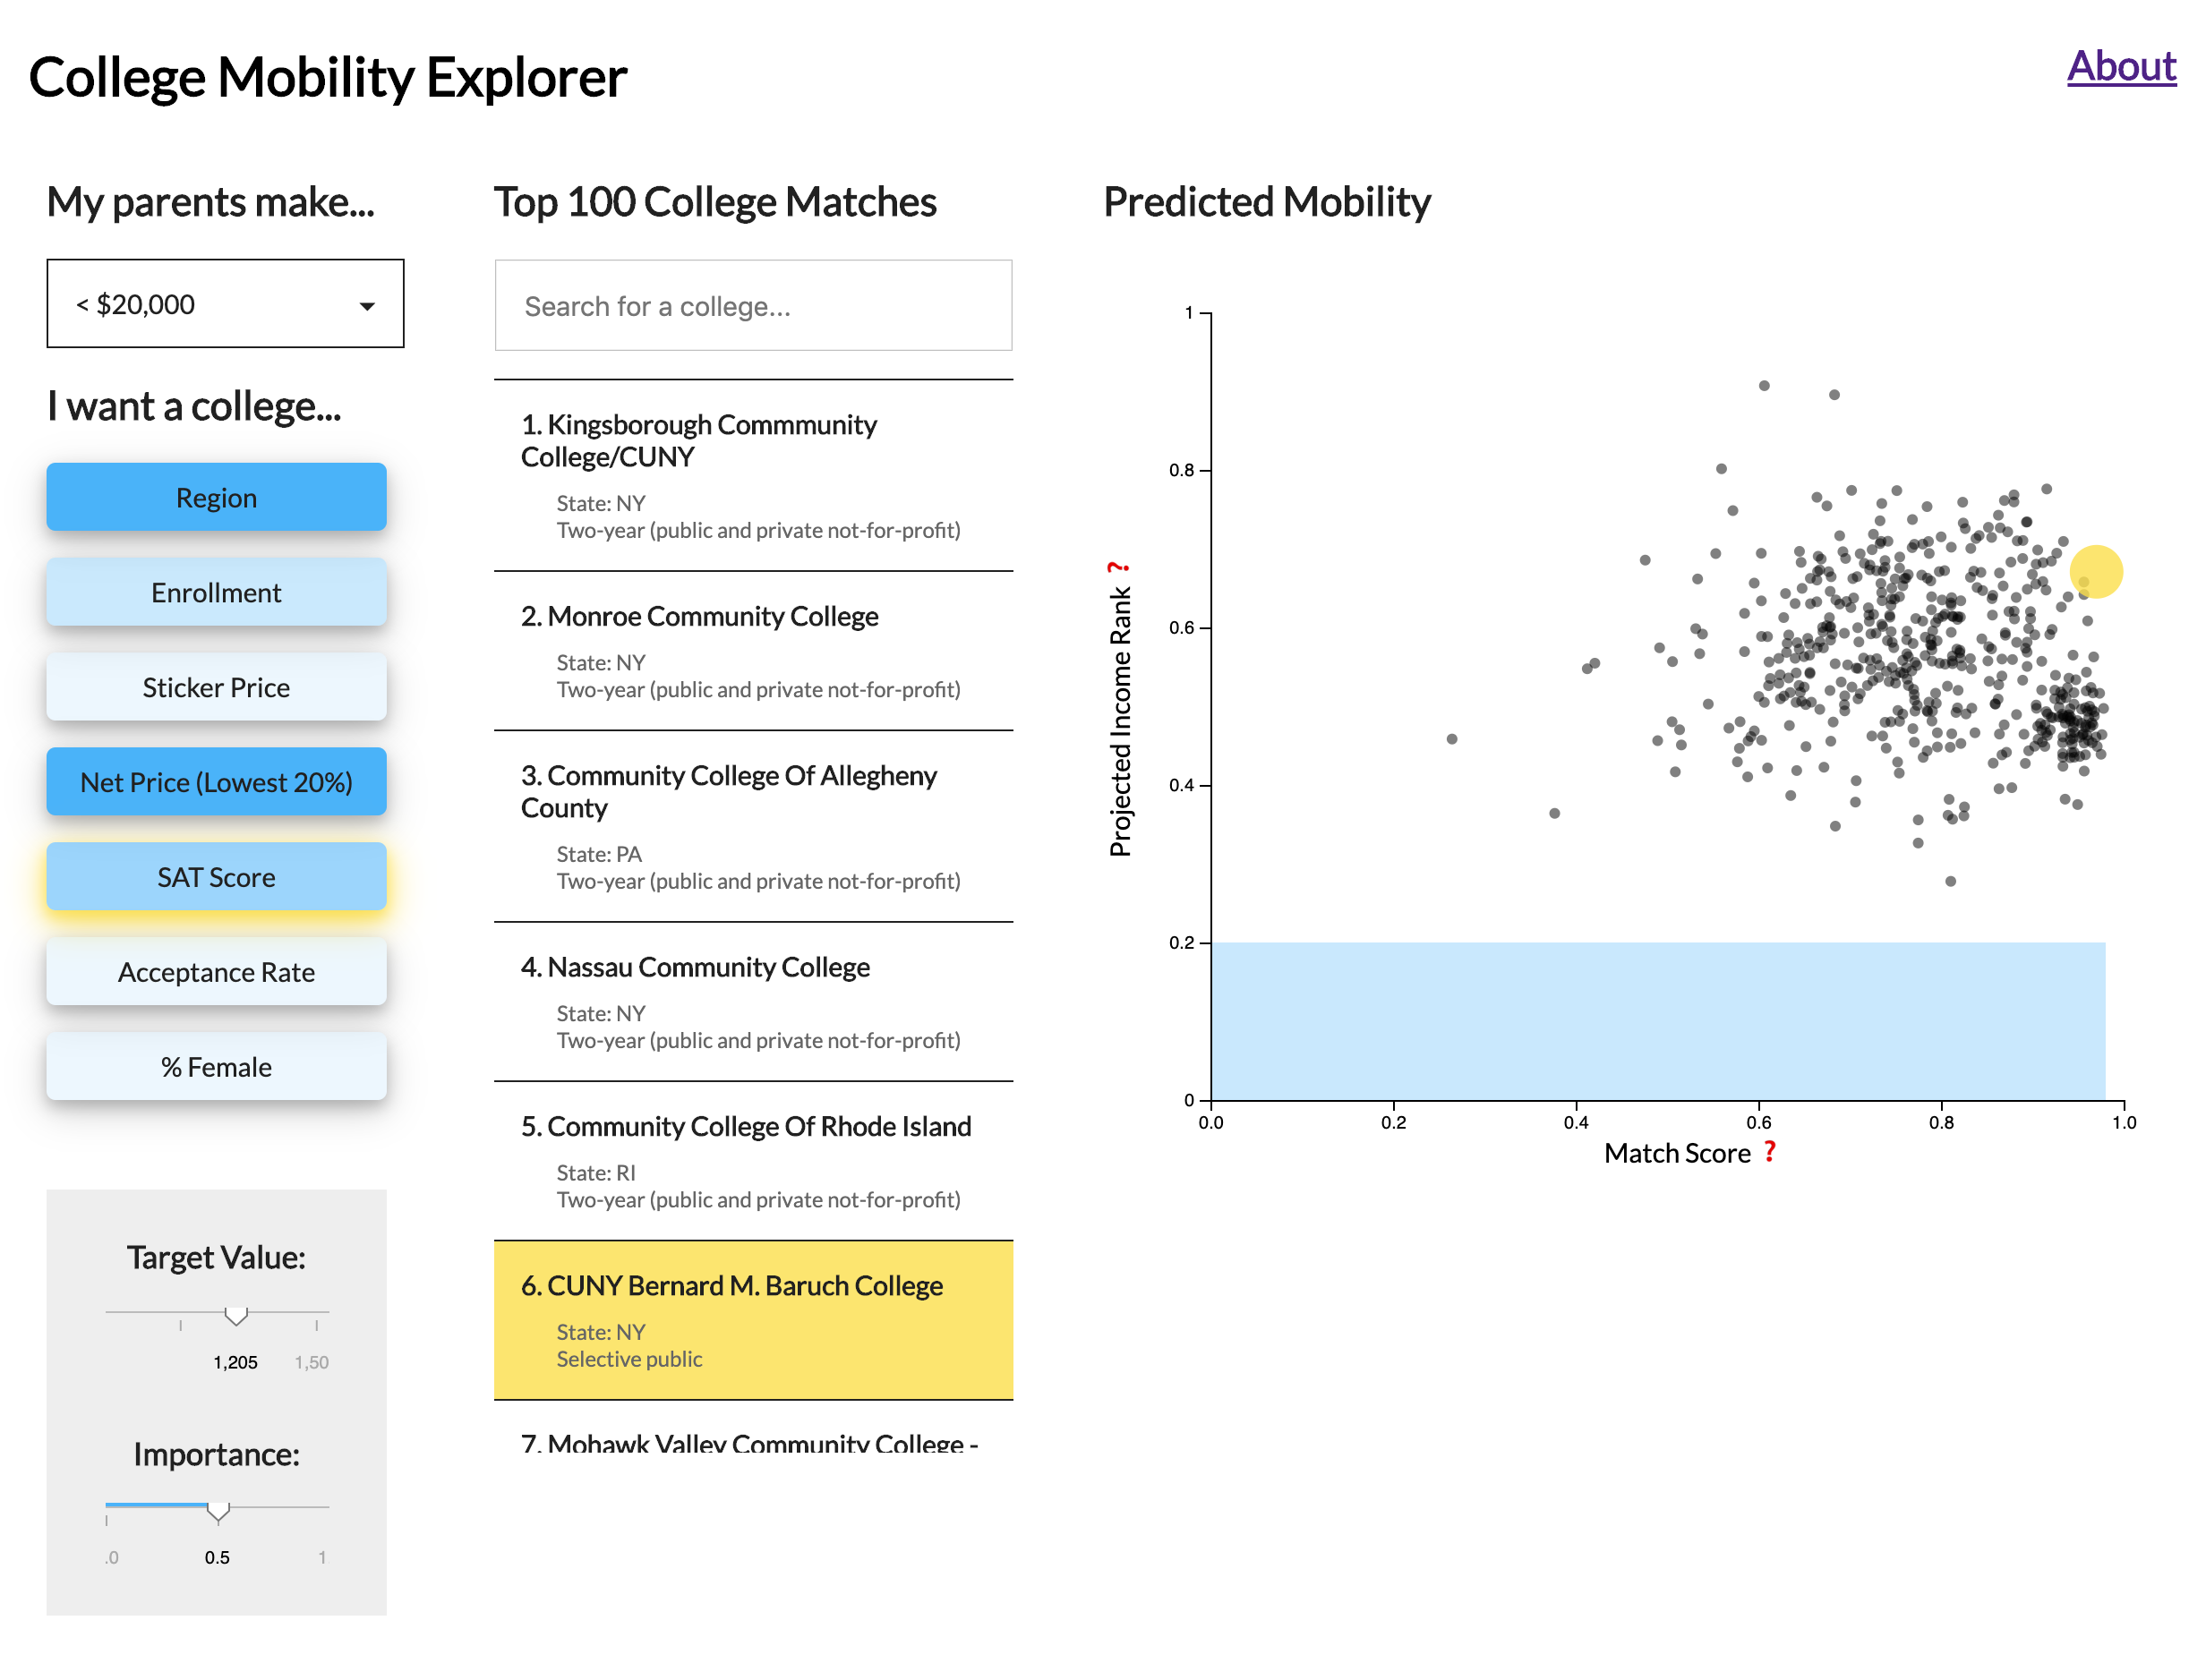
\includegraphics[width=\columnwidth]{cuny.png}
 \caption{Student A's results on feature selection and weighting.}
 \label{fig:cuny}
\end{figure}

Student A could then click through the first results on the top matches list and see from its location in the upper right section of the points on the scatter plot that \#6, CUNY Bernard M. Baruch College ranks highly on both match score for desired characters and income rank post-graduation. Student A could then scroll to the drill-down section, as visible in \autoref{fig:drilldown} and learn that the school has an enrollment of 14,082 students, price for low-income students of \$5,148, and admits students with an average SAT score of 1235. The pie-charts illustrate that the school has a fairly even gender representation, very high minority representation, and mostly business and STEM majors. This aligns with Student A’s desired features, so she could click on the website link and learn how to apply.

\begin{figure}[tbh]
 \centering
 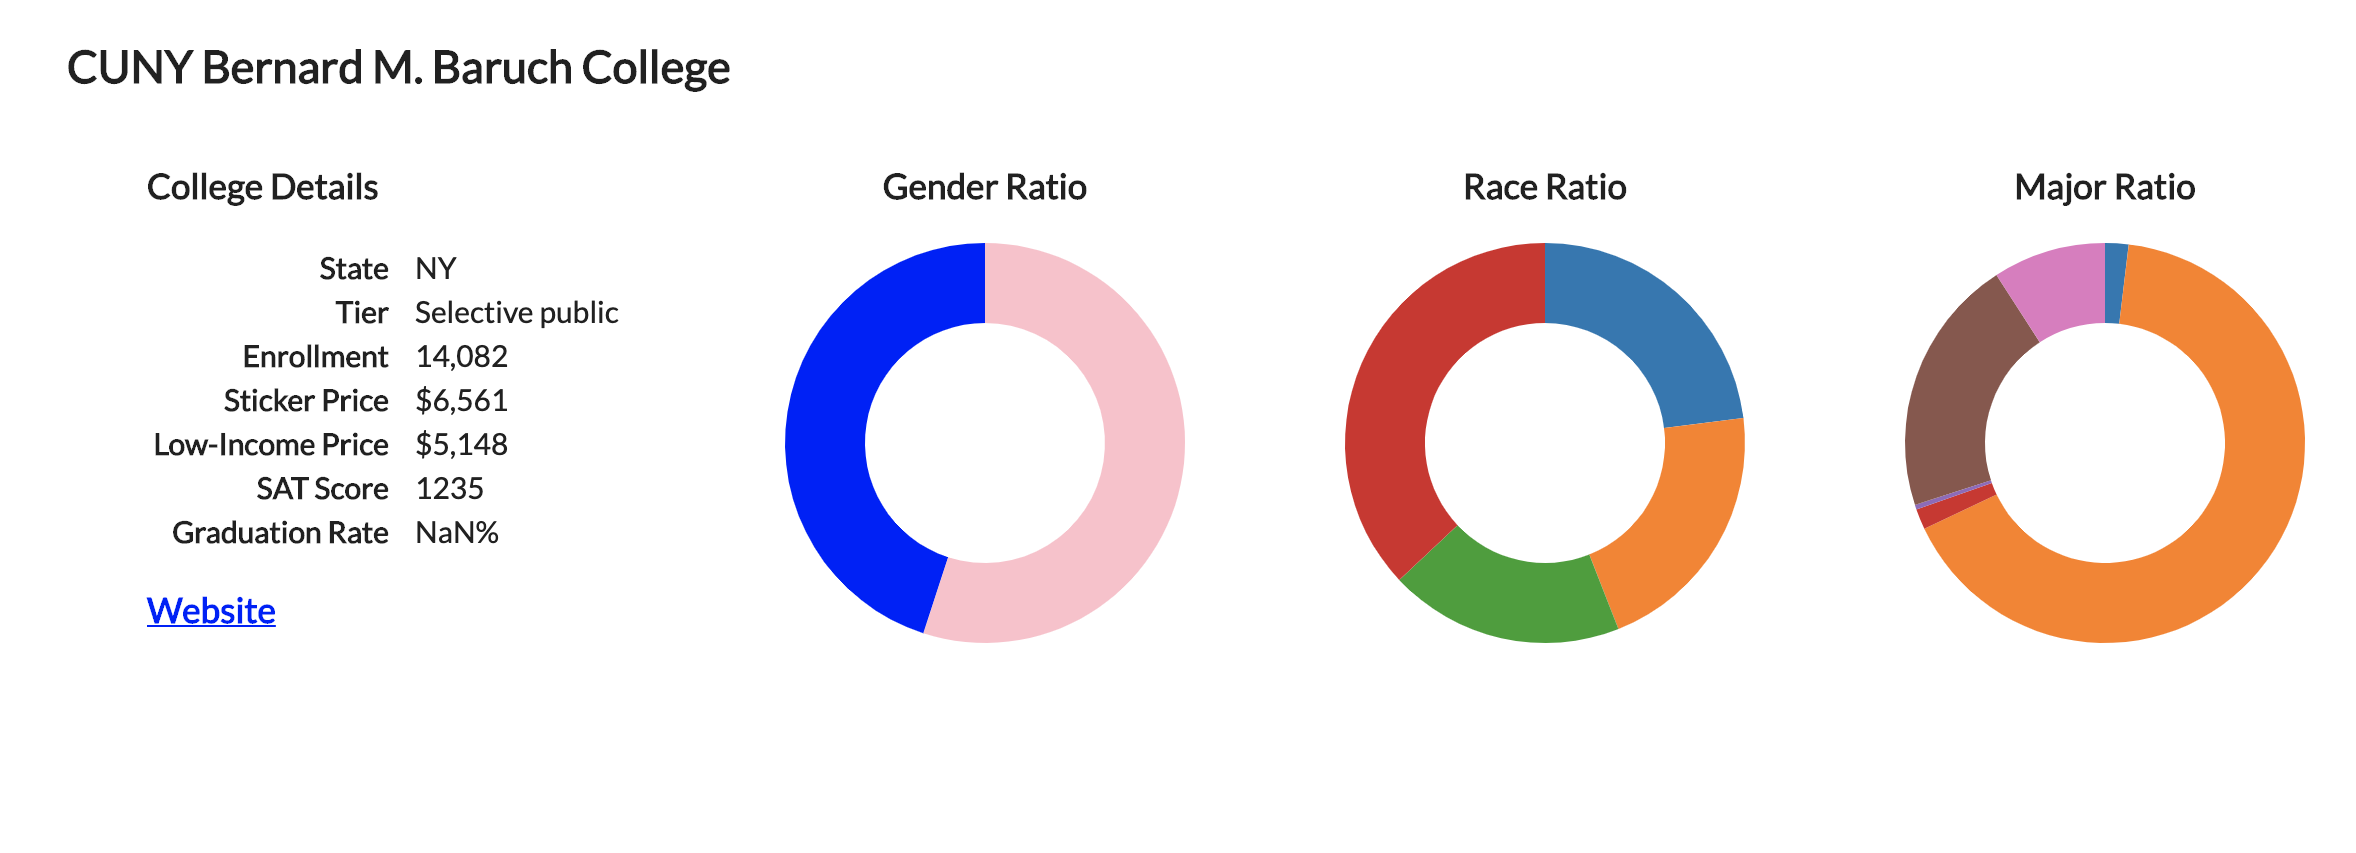
\includegraphics[width=\columnwidth]{drilldown.png}
 \caption{Student A's results after selecting CUNY Bernard M. Baruch College.}
 \label{fig:drilldown}
\end{figure}

\section{Discussion}
With the College Mobility Explorer, high-school students can explore colleges based on their desired features and parental incomes. Especially, upon the use of the scatter plot visualization, we glean a lot of interesting insights about different colleges as well as about the overall college selection process.

One interesting observation that confirms the Opportunity Insights' team's work is that on the whole, average end income does not vary drastically with starting income. This suggests that, although it may seem like richer students have a huge advantage coming into college, the overall effect does not translate into these students ending up with greatly higher incomes. For students from lower income quintiles, attending college is thus even more attractive as a method for income mobility.

Income also correlates with major and industries, as shown by specialized schools that tend to cluster and stand out with regards to this mobility measure. For example, schools that specialize in pharmacy (ex. MCPHS, Albany College of Pharmacy \& Health Sciences) have very high projected incomes regardless of starting income, but they do only offer one course of study. This puts them out of consideration of students with other conflicting interests.

With this idea, it is important to note that there is no objective ``best'' school to apply to, and neither axis unilaterally represents an ideal metric to prioritize when selecting colleges. Just selecting for the highest predicted income or for any trait specifically does not give a perfect college for anyone. On the contrary, college selection is ultimately a trade-off between a variety of factors, to which we can add mobility with the College Mobility Explorer.

Finally, upon this point, we also note that ``eliteness'' is one of these single-sighted factors. While name-recognition is an attractive factor, especially nowadays with the increasing ease of applying to many schools and competitiveness of admissions, it, just like any factor, does not single-handedly determine success. With this tool, we use objective information about the school as opposed to subjective ``eliteness'' or recognizability, to draw out schools that may not be as well-known, but may offer equivalent or even better mobility than schools that rely heavily upon their ``elite'' status to draw in students.

\section{Future Work}
We have several plans for future work on the College Mobility Explorer. First, there is more data on colleges that we would like to include. The average GPA of admitted students is a useful feature for prospective students to filter on. Average financial aid awarded by the school could be a relevant feature for low-income students especially, as well as a more exact representation of assistance provided by the school than the current proxy.

We also plan to expand the functionality of the feature selectors by allowing users to select a target range of values rather than just one specific value. This would be especially relevant for feature filters like “Sticker Price”, where users would be able to cap the amount of tuition they are willing to pay but equally award schools at that price or less. The match score would then be calculated based on outside distance to either the lower or upper ends of the ranges.

In addition, we plan to improve the performance of the interface such that we can list all schools under the college matches. Currently, the ranked list supports the top 100 school matches for the filter criteria, as those are most relevant to the search performed. With the over 2000 total schools, the ranked list cannot update in sync with adjusting filter target values and weights. However, we want to list all schools such that users are able to quickly find any specific institution.

Finally, we plan to include a more specific feature filter for selecting the geographic area of schools. We believe a measurement of how far the school is from the student’s home would be a relevant weighted metric for filtering schools. The dataset includes the zip code of each school as the most specific geographic marker. We plan to have an input for the student’s home address, and then lookup the distance between those two zip codes in miles as a distance measurement.

\section{Conclusion}
We have presented the College Mobility Explorer, an interface for discovery of well-suited colleges based on various financial and demographic features, while highlighting schools that provide high economic mobility opportunities. The interface provides actionable information to students seeking to apply to higher education institutions that can be most transformational to their financial situations. 

\acknowledgments{
The authors wish to thank Professor Arvind Satyanarayan, T.A. Soya Park, Caroline Dockes from the Opportunity Insights organization, and the 6.894 Spring 2019 class for their feedback, suggestions, and ideas regarding the creation of this project. }

\bibliographystyle{abbrv-doi}
\bibliography{template}
\end{document}
